\documentclass[aspectratio=169,12pt]{beamer}
\usepackage{amsmath}
\usepackage{amssymb}
\usepackage{xcolor}
\usepackage[most]{tcolorbox}
\usepackage{tikz}
\usepackage{graphicx}
\usepackage[sfdefault,lf]{FiraSans}
\renewcommand{\familydefault}{\sfdefault}
\setlength{\parindent}{0pt}
\setbeamertemplate{navigation symbols}{}
\setbeamertemplate{footline}{}
\setbeamertemplate{headline}{}
\definecolor{mmpageWhite}{HTML}{FCFBF7}
\definecolor{mmtanSoft}{HTML}{F7F5EF}
\definecolor{mmgreenDeep}{HTML}{244B2C}
\definecolor{mmgreenLeaf}{HTML}{5D8A56}
\definecolor{mmtext}{HTML}{163221}
\definecolor{mmanswerColor}{HTML}{306A3A}
\setbeamercolor{background canvas}{bg=mmpageWhite}
\setbeamercolor{normal text}{fg=mmtext,bg=mmpageWhite}
\newtcolorbox{AnsCard}[1][]{enhanced,breakable=false,colback=white,colframe=black,boxrule=1.5pt,arc=8pt,left=5pt,right=5pt,top=4pt,bottom=4pt,before skip=0pt,after skip=0pt,height=0.4\textheight,valign=center,#1}
\newcommand{\KoruIcon}{\raisebox{-0.2em}{
\includegraphics[height=1.05em]{img/header-logo.png}}}
\newcommand{\HoeIcon}{\raisebox{-0.2em}{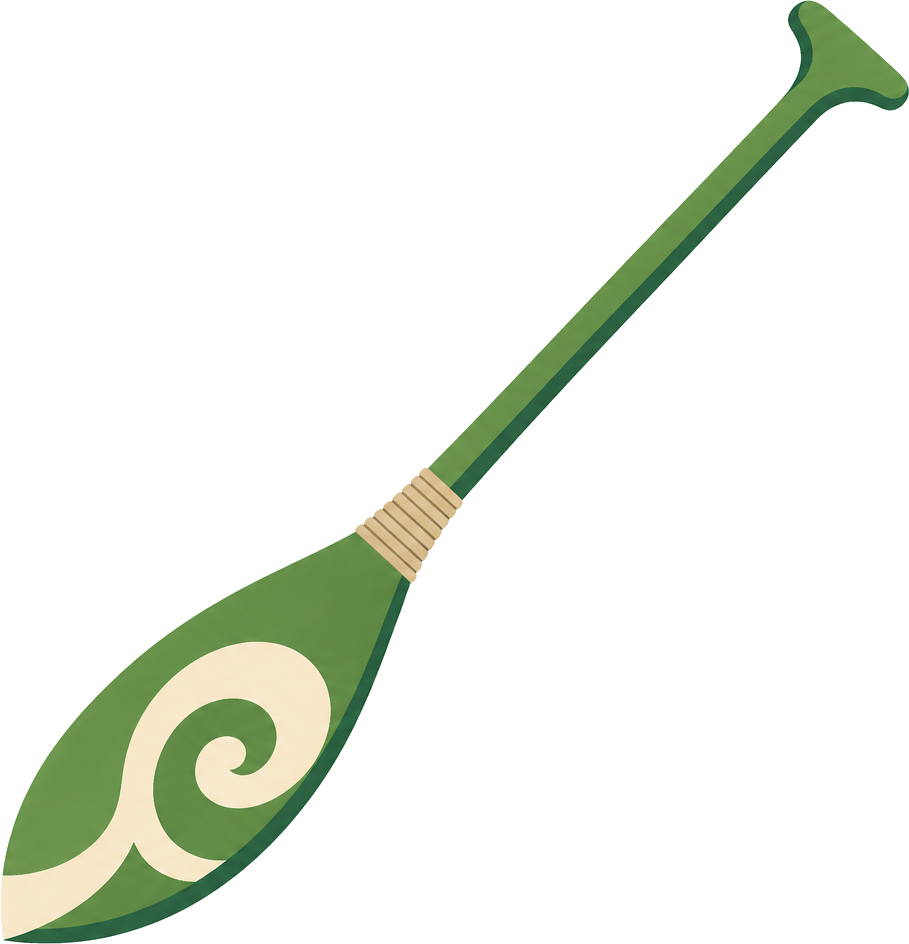
\includegraphics[height=1.05em]{img/hoe.png}}}
\newcommand{\ScaffoldIcons}[1]{\ifcase#1\or \HoeIcon\or \HoeIcon\hspace{0.22em}\HoeIcon\or \HoeIcon\hspace{0.22em}\HoeIcon\hspace{0.22em}\HoeIcon\fi}
\newcommand{\WorksheetTitle}[2]{%
  {\colorbox{mmtanSoft}{\parbox[c][2.2em][c]{0.975\linewidth}{%
    \hspace{0.25em}{\Large\bfseries\textcolor{mmgreenDeep}{#1}\hfill\ScaffoldIcons{#2}}}}
  \par\vspace{0.12em}{\color{mmgreenLeaf}\rule{\linewidth}{2.5pt}}\par\vspace{0.06em}}
}
\setbeamertemplate{background}{
 \begin{tikzpicture}[remember picture,overlay]
 \draw[black,line width=1.5pt,rounded corners=10pt]
 ([xshift=0.45cm,yshift=-0.45cm]current page.north west)
 rectangle
 ([xshift=-0.45cm,yshift=0.45cm]current page.south east);
 \end{tikzpicture}
}
\begin{document}
\begin{frame}[t]
\WorksheetTitle{Build Tasks - Answers}{1}
\vspace{-0.1em}
\begin{columns}[T,onlytextwidth]
\begin{column}{0.48\textwidth}\begin{AnsCard}\small\textcolor{mmgreenDeep}{\textbf{1. Cuboid 12$\times$8$\times$5 cm}}\\\vspace{0.1em}\textcolor{mmanswerColor}{\textbf{SA = 2(96+60+40) = 392 cm$^2$}}\end{AnsCard}\end{column}
\begin{column}{0.48\textwidth}\begin{AnsCard}\small\textcolor{mmgreenDeep}{\textbf{2. Box 1.2$\times$0.7$\times$0.5 m}}\\\vspace{0.1em}\textcolor{mmanswerColor}{\textbf{SA = 2(0.84+0.6+0.35) = 3.58 m$^2$}}\end{AnsCard}\end{column}
\end{columns}
\vspace{0.15em}
\begin{columns}[T,onlytextwidth]
\begin{column}{0.48\textwidth}\begin{AnsCard}\small\textcolor{mmgreenDeep}{\textbf{3. Cube SA = 384}}\\\vspace{0.1em}\textcolor{mmanswerColor}{\textbf{6s$^2$=384 $\to$ s$^2$=64 $\to$ s=8 cm}}\end{AnsCard}\end{column}
\begin{column}{0.48\textwidth}\begin{AnsCard}\small\textcolor{mmgreenDeep}{\textbf{4. Cuboid 15$\times$9$\times$4 cm}}\\\vspace{0.1em}\textcolor{mmanswerColor}{\textbf{SA = 2(135+60+36) = 462 cm$^2$}}\end{AnsCard}\end{column}
\end{columns}
\vspace{0.15em}
\begin{columns}[T,onlytextwidth]
\begin{column}{0.48\textwidth}\begin{AnsCard}\small\textcolor{mmgreenDeep}{\textbf{5. Four walls 5$\times$4$\times$2.4 m}}\\\vspace{0.1em}\textcolor{mmanswerColor}{\textbf{2(12)+2(9.6) = 43.2 m$^2$}}\end{AnsCard}\end{column}
\begin{column}{0.48\textwidth}\begin{AnsCard}\small\textcolor{mmgreenDeep}{\textbf{6. Walls+ceiling}}\\\vspace{0.1em}\textcolor{mmanswerColor}{\textbf{43.2 + 20 = 63.2 m$^2$}}\end{AnsCard}\end{column}
\end{columns}
\end{frame}
\begin{frame}[t]
\WorksheetTitle{Build Tasks - Answers}{1}
\vspace{-0.1em}
\begin{columns}[T,onlytextwidth]
\begin{column}{0.48\textwidth}\begin{AnsCard}\small\textcolor{mmgreenDeep}{\textbf{7. Cylinder r=3, h=10}}\\\vspace{0.1em}\textcolor{mmanswerColor}{\textbf{2$\pi$(3)(10)+2$\pi$(9) $\approx$ 244.92 cm$^2$}}\end{AnsCard}\end{column}
\begin{column}{0.48\textwidth}\begin{AnsCard}\small\textcolor{mmgreenDeep}{\textbf{8. Cylinder d=8, h=12}}\\\vspace{0.1em}\textcolor{mmanswerColor}{\textbf{r=4: 2$\pi$(4)(12)+2$\pi$(16) $\approx$ 401.92 m$^2$}}\end{AnsCard}\end{column}
\end{columns}
\vspace{0.15em}
\begin{columns}[T,onlytextwidth]
\begin{column}{0.48\textwidth}\begin{AnsCard}\small\textcolor{mmgreenDeep}{\textbf{9. Cylinder SA=471, r=5}}\\\vspace{0.1em}\textcolor{mmanswerColor}{\textbf{31.4h+157=471 $\to$ h=10 cm}}\end{AnsCard}\end{column}
\begin{column}{0.48\textwidth}\begin{AnsCard}\small\textcolor{mmgreenDeep}{\textbf{10. Pencil 20$\times$12$\times$8 mm}}\\\vspace{0.1em}\textcolor{mmanswerColor}{\textbf{SA = 2(240+160+96) = 992 mm$^2$}}\end{AnsCard}\end{column}
\end{columns}
\vspace{0.15em}
\begin{columns}[T,onlytextwidth]
\begin{column}{0.48\textwidth}\begin{AnsCard}\small\textcolor{mmgreenDeep}{\textbf{11. Cube 0.4 m}}\\\vspace{0.1em}\textcolor{mmanswerColor}{\textbf{SA = 6(0.16) = 0.96 m$^2$}}\end{AnsCard}\end{column}
\begin{column}{0.48\textwidth}\begin{AnsCard}\small\textcolor{mmgreenDeep}{\textbf{12. Cuboid w=5, h=7, SA=214}}\\\vspace{0.1em}\textcolor{mmanswerColor}{\textbf{2(12l+35)=214 $\to$ l=6 cm}}\end{AnsCard}\end{column}
\end{columns}
\end{frame}
\begin{frame}[t]
\WorksheetTitle{Build Tasks - Answers}{1}
\vspace{-0.1em}
\begin{columns}[T,onlytextwidth]
\begin{column}{0.48\textwidth}\begin{AnsCard}\small\textcolor{mmgreenDeep}{\textbf{13. Cube 2.5 cm}}\\\vspace{0.1em}\textcolor{mmanswerColor}{\textbf{SA = 6(6.25) = 37.5 cm$^2$}}\end{AnsCard}\end{column}
\begin{column}{0.48\textwidth}\begin{AnsCard}\small\textcolor{mmgreenDeep}{\textbf{14. Paint can label}}\\\vspace{0.1em}\textcolor{mmanswerColor}{\textbf{$\pi$dh $\approx$ 3.14$\times$10$\times$14 = 439.6 cm$^2$}}\end{AnsCard}\end{column}
\end{columns}
\vspace{0.15em}
\begin{columns}[T,onlytextwidth]
\begin{column}{0.48\textwidth}\begin{AnsCard}\small\textcolor{mmgreenDeep}{\textbf{15. Cylinder r=6, h=15}}\\\vspace{0.1em}\textcolor{mmanswerColor}{\textbf{SA $\approx$ 565.2+226.08 = 791.28 cm$^2$}}\end{AnsCard}\end{column}
\begin{column}{0.48\textwidth}\begin{AnsCard}\small\textcolor{mmgreenDeep}{\textbf{16. Room 6$\times$4.5$\times$2.8}}\\\vspace{0.1em}\textcolor{mmanswerColor}{\textbf{85.8-8 = 77.8 m$^2$}}\end{AnsCard}\end{column}
\end{columns}
\vspace{0.15em}
\begin{columns}[T,onlytextwidth]
\begin{column}{0.48\textwidth}\begin{AnsCard}\small\textcolor{mmgreenDeep}{\textbf{17. Cuboid 25$\times$15$\times$10}}\\\vspace{0.1em}\textcolor{mmanswerColor}{\textbf{SA = 2(375+250+150) = 1550 cm$^2$}}\end{AnsCard}\end{column}
\begin{column}{0.48\textwidth}\begin{AnsCard}\small\textcolor{mmgreenDeep}{\textbf{18. Tri prism B=20, P=24, h=10}}\\\vspace{0.1em}\textcolor{mmanswerColor}{\textbf{2(20)+24(10) = 40+240 = 280 cm$^2$}}\end{AnsCard}\end{column}
\end{columns}
\end{frame}
\end{document}
